\icode{E-EME-SI-L2-261121-005}
如图所示，正电荷均匀分布在半圆形绝缘细杆上，细杆上的电荷在圆心\(O\)处产生的电场强度大小为\(E\)。杆上的\(P\)、\(Q\)两点把杆分为长度相等的三部分，现在保持杆\(AP\)段和\(BQ\) 带电情况不变，但\(PQ\) 段均匀带上和之前电量相等的负电荷，则圆心\(O\)处的电场强度变为\paren[]

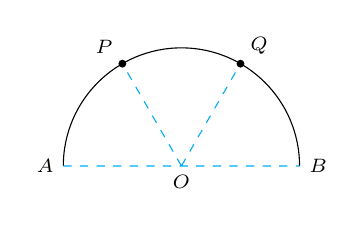
\begin{tikzpicture}[>=stealth,font=\scriptsize]
	\draw (-1.5,0)node[left]{\(A\)} arc(180:0:1.5)node[right]{\(B\)};
	\draw[dashed,cyan] (-1.5,0)--(1.5,0) (0,0)node[below,black]{\(O\)}--(60:1.5)node[above right,black]{\(Q\)} (0,0)--(120:1.5)node[above left,black]{\(P\)};
	\fill (60:1.5) circle(.05) (120:1.5) circle(.05);
\end{tikzpicture}
\begin{choices}
	\item \(\frac{E}{2}\)
	\item \( - \frac{E}{2}\)
	\item \(0\)
	\item \( - \frac{E}{3}\)
\end{choices}
\begin{answer}
	C\qquad 提示：
\end{answer}